\chapter{Word Embeddings}
\section{Introduction}
The main problem with the bag-of-words model is that it does not capture relations between words. In the bag-of-words model, each word or other feature of a text is represented by one dimension in a multidimensional space for representing the documents (we talk about one-hot representation [\cite{ref101}]). Each such dimension is independent of the others because it is represented by only one value which does not enable sharing some information across features. It is, therefore, not possible to say that, for example, the word football is more similar to the word soccer than to the word ballet.

On the other hand, when there are relatively few features and there are no correlations between them (or we do not want to take the correlations into consideration), one-hot representations can be more beneficial than alternative representations which somehow represent the correlations and reduce the sparseness typical of the bag-of-words model [\cite{ref101}].

To solve the problem where there is no similarity among words in the bag-of-words model, it would be possible to add other information to the existing words in a text, to better capture their context. Instead of keeping information, for example, the word is $A$, it is possible to store that the word is $A$, it's POS tag is $T$, the previous word is $B$, and the following word is $C$. This, however, increases the number of dimensions in the input space and requires the combination of possible feature components to be carefully selected.

Some of the modern representations of texts are based on the idea that similar words should have similar properties. This, however, cannot be achieved in the classic bag-of-words model. Thus, more than one dimension is needed to represent each word or feature. In this approach, each word is mapped to a continuous

\begin{displayquote}
I visited Brno last year. \\ 
He travelled from Brno to New York.\\ 
Brno has almost half a million inhabitants.\\ 
There are twenty nine districts in Brno.
\end{displayquote}

\hspace{-1.5em}\textbf{Figure 13.1:} Word Brno appearing in a few sentences. A reader can guess that Brno is a city even without ever hearing about it. This is because the word appears in the same or similar contexts as the names of cities the reader knows.\\[1em]

\hspace{-1.5em}multidimensional space which typically has a few hundred dimensions, which is much less than the number of dimensions in the bag-of-words model. The words are then embedded in this continuous vector space. We therefore talk about word embeddings.

Since the word vectors are usually found in an unsupervised training process, the dimensions are difficult to interpret. The vector can be understood as a vector of contextual features, because it is constructed based on the context in which the word appears. Anyway, similar words in this space are expected to be close to each other.

The basic idea of these alternative models is that words appearing in similar contexts usually have similar meaning. For an explanation, look at Figure 13.1. Here, a few sentences contain the not very well-known word, Brno. Despite this, a reader understands that it is very likely the name of a city. This is because similar sentences contain names of cities which the reader knows. These sentences typically talk about the number of inhabitants, districts, travelling directions, etc. All these aspects need to be somehow contained in a representation of a word; hence, so it is obvious that one dimension in a bag-of-words model is definitely not enough.

Similar words share some information; therefore, the values of their vector elements should be similar. They are thus located close to each other in the multidimensional space. Besides capturing the similarity between the words, models based on this principle also bring some additional advantages or possibilities. Because words are represented by vectors, vector operations can be performed with them, which can provide very surprising answers.

If a relationship exists between words A and B , and there is a similar relationship between words C and D , the offset of A and B , and C and D is also similar; see Figure 13.2. The relationship can be semantic, like the gender relation, or city-country relation as in Figure 13.2, but also syntactic like singular-plural, present tense-past tense, or base-comparative-superlative forms of an adjective [\cite{ref195}].

Probably the most famous example presented in [\cite{ref195}] says that\\
$vector("king") - vector("man") + vector("woman")$

\begin{figure}[H]
\begin{center}
  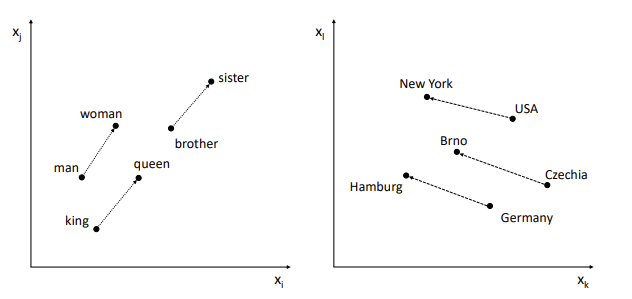
\includegraphics[width=\textwidth]{chapter/chapter13/figure13_2.png}
\captionsetup{labelformat=empty}
\caption{\textbf{Figure 13.2:} Examples of regularities in the word embeddings space.}
\label{fig13.2}
\end{center}
\end{figure}

will be very close to vector("queen") which captures the male/female relationship. The capital-of relation can be demonstrated with an example like

$$
{ vector("paris") - vector("france") + vector("poland") } \approx { vector("warsaw") }
$$

and a pluralisation relation by

$$
{ vector("cars") - vector("car") + vector("apple") } \approx { vector("apples"). }
$$[269]

Using word vectors can also significantly help in calculating true document similarities. When two sentences have a very similar meaning but use synonyms instead of the same words classic similarity measures will say that the sentences are not similar. When stop words are not taken into consideration, the sentences The queen visited the capital of US. and Elizabeth came to Washington in the USA. share no words. They, however, describe the same situation. In the space of word vectors, word pairs Elisabeth and queen and USA and US will be very close. This is the idea behind the Word Movers Distance (WMD) measure, which quantifies the dissimilarity between two documents as the minimum amount of distance that the embedded words of one document need to travel to reach the embedded words of another document, thus taking similarity of word vectors into consideration [\cite{ref157}].

\section{Determining the Context and Word Similarity}
Finding suitable values for the elements of the vectors representing words is based on the hypothesis stating that words in similar contexts have similar meanings [\cite{ref165}]. A key question is, what is the context of a word. A context can be\\
defined as a set of words that are, in some way, in a defined environment of the word. It might be the same document, sentence, or a piece of a text of some length (for example, five words to the left and five words to the right).

The simplest form of finding words with similar contexts is looking at the document-term matrix. If the matrix has $n$ rows ( $n$ is the number of documents) and $m$ columns ( $m$ is the number of terms), words with similar contexts have similar columns. In this case, the context are entire documents.

If the context is not the entire document, it is more common to use a word co-occurrence matrix instead of a document-term matrix. A word co-occurrence matrix is a square matrix where the rows and columns are labeled by the words. The elements of the matrix contain the frequencies with which the words cooccur.

A disadvantage of using raw frequencies in a term-term matrix is that some words with high frequencies (often stop words) tend to co-occur with many other words but are not very discriminative. Instead, it is better to somehow normalize the frequencies so that real relations between words become obvious. One of the more commonly used measures in this context is pointwise mutual information (PMI); see Section 14.3.2. It measures whether two words occur more often together than if they were independent. The values of PMI range from $-\infty$ to $+\infty$. Negative values are replaced by zeros because it can be problematical to interpret what it means that words co-occur less than by chance. The measure is biased towards low frequency words, so raising the probabilities to a number (e.g., 0.75) or adding one (Laplace smoothing) to all frequencies is often used [\cite{ref138}].

Both document-term matrices and word co-occurrence matrices usually have many rows and columns (tens of thousands) and their vectors are sparse (many zeros). It is desirable to use representations where the vectors have different properties. They should be shorter so that using them in a machine learning task is easier (less parameters need to be learned) and most of the values are not zeros (i.e., the vectors are dense).

Popular approaches leading to generating dense vectors include models using global matrix factorization like Latent Semantic Analysis (LSA) or Latent Dirichlet Allocation (LDA) and models learned by neural networks using a small context window (where word 2 vec is probably the most popular). In many situations, the models based on neural networks perform better than LSA in the preservation of linear regularities among words (important for the word analogy task, for example) and are computationally more efficient than LDA . On the other hand, global methods like LSA can efficiently leverage statistical information unlike local methods like $word2vec$ [\cite{ref195}, \cite{ref214}].

\section{Context Windows}
Short pieces of text in a neighbourhood of a word are quite popular to define the context. Three context types can be distinguished according to what is being considered [\cite{ref101}]:

\begin{itemize}
  \item Continuous bag-of-words - the context is represented by words from a window where no order or positions are considered (e.g., the context of X is $\mathrm{A}, \mathrm{B}, \mathrm{C}$, and D ).
  \item Positional - the relative positions of other words are considered (e.g., the context of X is A two positions to the left, C one position to the left, D one position to the right, and C two positions to the right from X ).
  \item Dependency - syntactic connections to the word are considered (e.g., A is subject of $\mathrm{X}, \mathrm{B}$ is object of X ).
\end{itemize}

When the context is determined by a window surrounding a word, the windows size has an impact on the learned embeddings. When smaller context windows are used ( $1-3$ words), more syntactic and functional similarities are found. Longer windows ( $4-10$ words) discover more semantic similarities [\cite{ref138}].

The content of the window can also be modified before training. The words can have different weights assigned according to the distance to the word for which they define the context (this can be achieved through sampling). Words of high frequency can be removed before training. Here, two cases can be distinguished - the words are removed before defining their contexts (which means that the context window enlarges, words further from the predicted word will be included in the context), or after creating the windows (the context window has the same size). Rare words can also be removed; this, however, has little impact on the quality of learned embeddings [\cite{ref166}].

\section{Computing Word Embeddings}
Supervised methods require annotated data for a specific task; for example, texts with part of speech tags for the part of speech tagging task. Then, the embeddings are trained towards the given goal and can capture information that is relevant for the task. The created embeddings can be successfully used for a related task (like syntactic parsing) for which there is not enough labeled data. The embeddings learned in one task can be also transferred to another task and improved with some labeled data from the other task [\cite{ref101}].

Unsupervised methods for word embeddings training do not require annotated data. Their only goal is to compute embeddings. The embeddings are usually learned in the task of predicting a word given its context, or deciding whether, given examples of real and randomly created word-context pairs, a word\\[0pt]
can belong to a context [\cite{ref101}]. Large corpora that are available can be used for training instead of annotated texts. The learned embeddings capture general syntactic and semantic relationships and can be applied in a wide variety of tasks.

There are a few famous methods that can be used to compute word embeddings:

\begin{itemize}
  \item \textbf{Neural language models}. Dense vector representations (embeddings) can be learned in a neural network (usually the first layer) that is provided with one-hot vectors [101]. The first works producing word embeddings used neural networks for language modeling. In a neural probabilistic language model [\cite{ref21}], $k$ words from a text were taken as an input and the probabilities of the following word were calculated using softmax; see Figure 13.4. Collobert et al. [\cite{ref57}] used a window around a word instead of several preceding words to predict a correct word. They also replaced probability calculations with the assignation of higher scores to correct words and lower scores to incorrect words. Vectors representing the words are concatenated and processed by a neural network with one hidden layer.
  \item \textbf{Word2vec}. Word2vec is a family of methods proposed by Tomáš Mikolov that drew the NLP community to neural language models. The prediction in word2vec has two forms - predicting the word based on its context (the Continuous bag-of-words or CBOW approach), and predicting the context for a word (the Skip-gram approach); see Figure 13.4. The input and output in both cases are one-hot encoded vectors. Word2vec tried to eliminate the problems of the previous neural language models with computational complexity. In the training phase, a neural network uses a linear activation function instead of the sigmoid function, which is typical for a multilayer perceptron, and the logarithm of the probability of predicting the word or its context context is maximized [\cite{ref194}].\newline
As Levy and Goldberg [165] found, learning word vectors using the skipgram model with negative sampling (artificially created pieces of text that are added to the training set should be distinguished from real texts) are an implicit factorization of a positive pointwise mutual information matrix of word-context pairs.\\
  \item \textbf{GloVe}. GloVe is a model developed at Stanford University. Unlike word2vec, which learns word vectors directly, GloVe uses information about global co-occurrences of words. It uses word vectors in the task of predicting the probability with which two words co-occur. More precisely, the ratios of word co-occurrence probabilities are predicted as the relationship between two words is examined by studying the ratio of cooccurrences with other, so called, probe words. The probabilities can be

\begin{figure}[H]
\begin{center}
  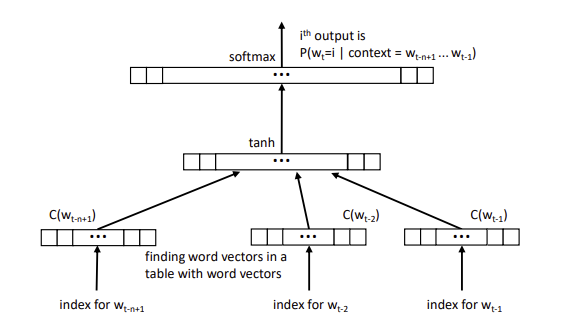
\includegraphics[width=0.8\textwidth]{chapter/chapter13/figure13_3.png}
\captionsetup{labelformat=empty}
\caption{\textbf{Figure 13.3:} The architecture of a probabilistic neural language model. $C(w_i)$ is a word vector corresponding to word $i$ [\cite{ref21}].}\end{center}
\label{fig13.3}
\end{figure}

\begin{figure}[H]
\begin{center}
  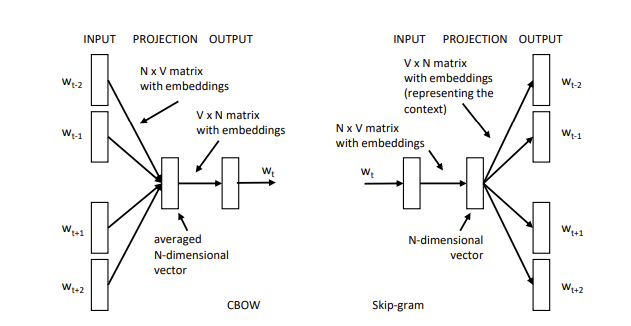
\includegraphics[width=0.8\textwidth]{chapter/chapter13/figure13_4.png}
\captionsetup{labelformat=empty}
\caption{\textbf{Figure 13.4:} The architectures of neural networks for training word embeddings using the
CBOW and Skip-gram approaches. $V$ is the size of the vocabulary, $N$ is the size of word
vectors, $w_i$ are one-hot encoded vectors of size $V$ containing indices of the given words [\cite{ref195}] [\cite{ref276}].}
\label{fig13.4}
\end{center}
\end{figure}

calculated from a term-term matrix created from a corpus. The prediction is made by a function that takes word vectors as the input. The word vectors are calculated in the process of word co-occurrence matrix factorization using stochastic gradient descent which is a process that can be parallelized [\cite{ref214}]. Compared to word2vec, the training is faster but it requires more memory.

  \item \textbf{fastText}. Most of the techniques for learning word embeddings ignore sub-word information (prefixes, suffixes) which is very important for morphologically rich languages with many rare words. The fastText model, which is derived from word 2 vec, treats each word as a bag of character n -grams where the vectors are associated at the n -gram level. The vector for a word is calculated as the sum of n -gram vectors. This also enables creating vectors for words that are not in the training data [\cite{ref28}].
\end{itemize}


When generating embeddings is a part of a neural network, the vectors can be initialized randomly as in the case of other model parameters. The values can be sampled uniformly from a fixed interval centered at zero (for example, the Xavier method samples the values from the interval $\left[-\frac{\sqrt{6}}{\sqrt{n_{i}+n_{o}}},+\frac{\sqrt{6}}{\sqrt{n_{i}+n_{o}}}\right]$, where $n_{i}$ and $n_{o}$ are the sizes of input and output), or from a zero-mean normal distribution with the standard deviation varying from 0.001 to 10 [148].

Instead of training, word vectors embeddings pre-trained on many different collection can be found. The collections are trained on sources like Wikipedia articles, tweets, Common Crawl, Google news and others.

\section{Aggregation of Word Vectors}
To represent larger pieces of text (sentences, paragraphs, documents), word vectors need to be aggregated somehow. Otherwise, the text can be viewed as a bag of embedded words with a variable length [56]. Many algorithms, however, require fixed length vectors. The fixed length vectors can be an input to, for example, classification or clustering algorithms instead of document vectors from the bag-of-words model.

Simple aggregation approaches use, for example, the sum, average, or a weighted average (using tf-idf wights) of the word vectors [66, 195].

During training word vectors, it is generally expected that the vectors should help in predicting other words in the given context. A similar idea is used by Le and Mikolov [\cite{ref162}] in their Paragraph Vector algorithm. A larger piece of text, here a paragraph, should be useful in predicting other words too. The paragraph vector then behaves like another word in the prediction task. It represents the missing information from the current context and acts as a memory of the topic of the paragraph. Word vectors are shared across all paragraphs while the paragraph vectors are not.

A recursive neural network architecture to aggregate words vectors was proposed in [\cite{ref253}]. The method requires parsing and thus works on a sentence level.

Another method to aggregate and compress the variable-size word embedding sets to binary hash codes through Fisher kernel and hashing methods was proposed in [\cite{ref290}].

\section{An Example}
To train a word $2 v e c$ model, the wordVectors library can be used. At this moment, it is not in the CRAN archive. It is, therefore, necessary to download it from github using devtools.

\begin{verbatim}
library(devtools)
install_github("bmschmidt/wordVectors")
library(wordVectors)
\end{verbatim}

The author of wordVectors demonstrates the functionality on texts from cookbooks from Michigan State University. The archive with cookbooks is downloaded, stored as cookbooks.zip and unzipped to directory cookbooks. The directory will contain more than 70 text files with some cookbooks.

\begin{verbatim}
download.file("http://archive.lib.msu.edu/
        dinfo/feedingamerica/cookbook_text.zip",
    "cookbooks.zip")
unzip("cookbooks.zip", exdir="cookbooks")
\end{verbatim}

To train a model, a text file containing the texts is needed. This file can be prepared in may different ways. The wordVectors library provides function prep\_word2vec() that determines a file or directory with the original texts (parameter origin), the output file name (destination), information about ngram handling (parameter bundle\_ngrams - if the value is greater than 1, joins together common n-grams into a single word), and the possibility to lowercase the text (lowercase).

\begin{verbatim}
prep_word2vec(origin="cookbooks",
    destination="cookbooks.txt",
    lowercase=TRUE,
    bundle_ngrams=2)
\end{verbatim}

Subsequently, a word2vec model can be trained using the train\_word2vec () function on the created data file. Training parameters include the size of word vectors (parameter vectors), the size of the window around a word (window), the number of threads to run the training process on (threads), specification about whether to use the CBOW or skip-gram approach ((cbow), the minimal frequency of a word in the corpus to be included in the samples (min\_count),\\
the number of passes over the corpus in training (iter), or the number of negative samples in the skip-gram approach (negative\_samples). The word vectors are written to an output file with in binary form (parameter destination). The function returns an object containing word vectors.

\begin{verbatim}
model <- train_word2vec(train_file="cookbooks.txt",
    output_file="cookbook_vectors.bin",
    vectors=200,
    threads=4,
    window=12,
    iter=5,
    negative_samples=0)
\end{verbatim}

Individual word vectors can be accessed through a string containing the word of interest. In the following example, we are using the function closest\_to() to find words most similar to steak and cheese (two ingredients that are mentioned in cookbooks).
\begin{verbatim}
> x <- model["steak", ]
> closest_to(model, x)
                      word similarity to x
1 steak              1.0000000
2 beefsteak          0.7224785
3 rump_steak         0.6747437
4 porterhouse_steak  0.6517441
5 steaks             0.6482365
6 sirloin            0.5996025
7 planked_sirloin    0.5941793
8 roast_beef         0.5836023
9 tenderloin         0.5827629
10 broil             0.5745636
>
> x <- model["cheese", ]
> closest_to(model, x)
                      word similarity to x
1 cheese             1.0000000
2 swiss_cheese       0.6298522
3 edam               0.6113659
4 emmenthaler        0.5890561
5 stilton            0.5821470
6 cheshire           0.5780776
7 gruy_232           0.5679422
8 kase               0.5519617
9 cottage_cheese     0.5487433
10 neufchatel        0.5484801
\end{verbatim}

We can also try some vector arithmetic - we want to know what is to pork as steak is to beef.

\begin{verbatim}
> x <- model["steak", ] - model["beef", ] + model["pork", ]
> closest_to(model, x)
# this is also possible:
# closest_to(model, ~"steak"-"beef"+"pork")
\end{verbatim}

\begin{center}
\begin{tabular}{|l|l|l|}
\hline
\multirow[b]{2}{*}{1} & \multicolumn{2}{|r|}{word similarity to x} \\
\hline
 & steak & 0.7268982 \\
\hline
2 & pork & 0.6755440 \\
\hline
3 & steaks & 0.5458622 \\
\hline
4 & bacon & 0.5458076 \\
\hline
5 & chops & 0.5364155 \\
\hline
6 & pork\_chops & 0.5351922 \\
\hline
7 & broil & 0.5095040 \\
\hline
8 & broiled & 0.4904118 \\
\hline
9 & beefsteak & 0.4878030 \\
\hline
10 & ham & 0.4817139 \\
\hline
\end{tabular}
\end{center}

Another example will reveal what can be made from apples as butter is made from milk.

\begin{verbatim}
> x <- model["butter", ] - model["milk", ] + model["apple", ]
> closest_to(model, x)
            word similarity to x
1 apple 0.6531934
2 apples 0.5038533
3 \text { tart } 0 . 4 6 7 2 2 1 8
4 butter 0.4625596
5 \text { lamb's_sweetbreads } 0 . 4 5 8 1 4 0 0
6 pie 0.4531101
7 apple_marmalade 0.4487496
8 8 7 2 0 . 4 3 6 2 9 2 7
9 sauce 0.4331859
10 compote 0.4307663
\end{verbatim}

The following two examples try to show some syntactic regularities (plural/singular and base/continuous form of a verb).

\begin{verbatim}
> x <- model["apples", ] - model["apple", ] + model["pear", ]
> closest_to(model, x, n=5)
                    word similarity to x
1 pear 0.8229101
2 pears 0.6867127
3 apples 0.6411531
4 peaches 0.6117798
5 \text { apricots } 0 . 5 9 1 1 2 4 9
\end{verbatim}

\begin{verbatim}
> x <- model["baking", ] - model["bake", ] + model["cook", ]
> closest_to(model, x)
            word similarity to x
1 cook 0.5258886
2 cooking 0.4665998
3 roasting 0.4510705
4 stewing 0.4445075
5 baking 0.4195846
\end{verbatim}

GloVe vectors can be learned with the text2vec package. In our example, the same text data (cookbooks) will be used.

\begin{verbatim}
library(text2vec)
# all files with cookbooks
file_list <- list.files(path='cookbooks', pattern="*.txt")
for (f in file_list) {
    # creating a full name including file and directory names
    fullname <- paste("cookbooks", "/", f, sep="")
    # reading all lines from a file
    t <- readLines(fullname, n=-1)
    # appending the cookbook to all texts
    text <- append(text, t)
}
# creating tokens from the text
tokens <- word_tokenizer(text)
# creating an iterator over the list of character vectors
\end{verbatim}

\begin{verbatim}
# which are the documents being processed
it <- itoken(tokens, progressbar=TRUE)
# creating the vocabulary using the iterator
v <- create_vocabulary(it)
# filtering out too rare words
v <- prune_vocabulary(v, term_count_min=3)
# a function mapping words to indices, it is later used
# to create a term co-occurrence matrix
vectorizer <- vocab_vectorizer(v)
# creating a term-co-occurrence matrix from windows
# of size 5 words to the left and right from a word
tcm <- create_tcm(it, vectorizer,
        skip_grams_window=10,
        skip_grams_window_context="symmetric")
# creating GloVe word vectors:
# - creating an object for a GloVe model
glove <- GlobalVectors$new(word_vectors_size=300,
        vocabulary=v,
        x_max=10)
# - fitting the model to a term-co-occurrence matrix
# (10 iterations of stochastic gradient descent, stopping
# when two subsequent iterations bring an improvement less
# than convergence_tol); the model learns vectors for main
# as well as for context words
vectors_main <- glove$fit_transform(tcm,
            n_iter=10,
            convergence_tol=0.01)
vectors_context <- glove$components
# - the sum of main and context vectors is calculated
word_vectors <- vectors_main + t(vectors_context)
\end{verbatim}

Now, we can query the model to see some regularities in the learned word vectors. To calculate similarities between rows of two matrices, function sim2() from package text2vec is used. The first parameter is the matrix with word vectors, the second is a row related to one word. To maintain the matrix type for the row, parameter drop is set to FALSE.

\begin{verbatim}
# calculating cosine similarities to word "beef"
> cos_sim <- sim2(x=word_vectors,
+ y=word_vectors["beef", , drop = FALSE],
+ method="cosine",
+ norm="l2")
# looking at five most similar words
> head(sort(cos_sim[, 1], decreasing=TRUE), 5)
\end{verbatim}

\begin{center}
\begin{tabular}{rrrrr}
beef & veal & meat & mutton & pork \\
1.0000000 & 0.7188874 & 0.6961990 & 0.6873831 & 0.6791247 \\
\end{tabular}
\end{center}

\begin{verbatim}
# finding out, what is to pork as steak is to beef
> y <- word_vectors["steak", , drop = FALSE] -
+ word_vectors["beef", , drop = FALSE] +
+ word_vectors["pork", , drop = FALSE]
> cos_sim <- sim2(x=word_vectors,
+ y=y,
+ method="cosine",
+ norm="l2")
> head(sort(cos_sim[, 1], decreasing=TRUE), 5)
\end{verbatim}

\begin{center}
\begin{tabular}{rrrrr}
steak & pork & bacon & chops & lard \\
0.7276466 & 0.6033111 & 0.3629336 & 0.3597848 & 0.3501749 \\
\end{tabular}
\end{center}
